\documentclass[10pt]{report}
\usepackage{./EE703handout}
\usepackage{tikz}
\usepackage{pgfplots}
\usetikzlibrary{decorations.pathmorphing}
\usepackage{mathtools}
\usepackage{subfig}
\usepackage{hyperref}
\usepackage{enumitem}
\usepackage{verbatim}
\usepackage{amssymb}
\usetikzlibrary{arrows,backgrounds,shapes,matrix,positioning,fit}
\setlength{\textheight}{9.4in}     % 9.4in
\setlength{\textwidth}{6.3in}      % 6.3in
\setlength{\parindent}{0mm}
%\setlength{\parskip}{3mm}
\setlength{\oddsidemargin}{0.0in}  % 0.0in
\setlength{\topmargin}{-0.0in}  % 0.0in
\setlength{\headheight}{0.0in}  % 0.0in


\begin{document}
\handout{}{Due Date: October 3, 2013}{Assignment 3}
\begin{enumerate}
  \item Consider the following hypothesis testing problem.
    \begin{equation*}
      \begin{array}{lll}
        H_1 : & Y_1 = A+N_1,& Y_2 = N_2 \\
        H_0 : & Y_1 = N_1,& Y_2 = N_2 
      \end{array}
    \end{equation*}
    where $A >0$, $\mathbf{Y} \sim N(\mathbf{m}_i,\mathbf{C})$ under hypothesis $H_i$, $\mathbf{Y} = \begin{bmatrix} Y_1 & Y_2 \end{bmatrix}^T$, $\mathbf{m}_0 = \begin{bmatrix} 0 & 0 \end{bmatrix}^T$, $\mathbf{m}_1 = \begin{bmatrix} A & 0 \end{bmatrix}^T$, $\mathbf{C} = \sigma^2 \begin{bmatrix} 1 & \rho \\ \rho & 1 \end{bmatrix}$. Show that $Y_2$ is a relevant statistic by deriving the following conditional densities.
    \begin{eqnarray*}
      p(y_2|y_1,H_0) & = & \frac{1}{\sqrt{2\pi(1-\rho^2) \sigma^2}} e^{-\frac{(y_2-\rho y_1)^2}{2(1-\rho^2)\sigma^2}},\\ 
      p(y_2|y_1,H_1) & = & \frac{1}{\sqrt{2\pi(1-\rho^2) \sigma^2}} e^{-\frac{[y_2-\rho (y_1-A)]^2}{2(1-\rho^2)\sigma^2}}
    \end{eqnarray*}
  \item $M$ signals $s_1(t), s_2(t), \ldots, s_M(t)$ which are nonzero for $0 \leq t \leq T$ are transmitted over an AWGN channel. Each signal is identical to all the others in the interval $[t_1,t_2]$ where $0 < t_1 < t_2 < T$. Show that the optimal receiver can ignore the signal received in the interval $[t_1,t_2]$ in taking its decision.
  \item A pulse $p(t)$ which is nonzero for $0 \leq t <T$ is transmitted through a channel which adds WGN $n(t)$ having PSD $\sigma^2$ and also induces a random delay $D$ as shown in the figure below. If the delay $D$ is equally likely to be $0$, $T$ or $2T$, what is the best estimator for the delay?
    \begin{figure}[h]
      \centering
        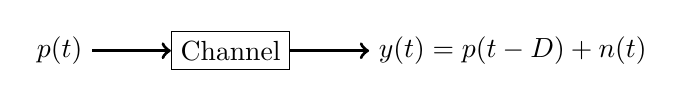
\begin{tikzpicture}[scale=1.0,transform shape]
          \node at (0,0) (pt) {$p(t)$};
          \node[rectangle, draw, right=1 of pt] (plus) {Channel};
          \node[right=1 of plus] (y) {$y(t) = p(t-D) + n(t)$};
          \draw[->,very thick] (plus) -- (y);
          \draw[->,very thick] (pt) -- (plus);
        \end{tikzpicture}
    \end{figure}
  \item Consider the $M$-ary hypothesis testing problem in AWGN where $s_i(t) = A_ip(t)$ for some distinct scalars $A_i \in \mathbb{R}$ and unit energy pulse $p(t)$ which is nonzero for $0 \leq t \leq T$.
    \begin{equation*}
      \begin{array}{ccc}
          H_1 & : & y(t) = s_1(t) + n(t) \\
          H_2 & : & y(t) = s_2(t) + n(t) \\
          \vdots &   &  \vdots          \\
          H_M & : & y(t) = s_M(t) + n(t) \\
      \end{array}
    \end{equation*}
  If all the hypotheses are equally likely, show that the optimal receiver compares the output of a matched filter to a set of thresholds.
\end{enumerate}
\end{document}
